
{
\date{René Magritte, Untitled}
\usebackgroundtemplate{
\includegraphics[width=\paperwidth,height=\paperheight]{img/matchers/part.jpg}}
\part{Matchers}
}

\begin{frame}[fragile]{New Assertion: \texttt{assertThat(\dots)}}
    \begin{itemize}
        \item New \texttt{Assert} methods:
    \begin{lstlisting}
<T> void assertThat(T actual, Matcher<T> matcher)
<T> void assertThat(String reason, T actual, Matcher<T> matcher)
\end{lstlisting}
        \item Parameters:
        \begin{description}[matcher]
            \item[reason]  description displayed when assertion fails (optional)
            \item[actual]  actual value
            \item[matcher] Hamcrest matcher that checks the actual value
        \end{description}
    \end{itemize}
\end{frame}

\begin{frame}[fragile]{Increased Readability}
    \only<1>{\javainputlisting[firstline=6]{hamcrest}{BetterReadability}}
    \only<2|handout:0>{\javainputlisting[firstline=6,emph={withoutMatchers,assertEquals}]{hamcrest}{BetterReadability}}
    \only<3|handout:0>{\javainputlisting[firstline=6,emph={withMatchers,assertThat}]{hamcrest}{BetterReadability}}
    \only<4|handout:0>{\javainputlisting[firstline=6,emph={is}]{hamcrest}{BetterReadability}}
    \begin{itemize}
        \item No more guessing about order of arguments
        \item Often more readable than traditional assertions
    \end{itemize}
\end{frame}

\begin{frame}[fragile]{Combining Matchers}
	Matchers are easily combined:
	\javainputlisting[firstline=20,lastline=21,tabsize=1]{hamcrest}{WithMatchers}
\end{frame}

\begin{frame}[fragile]{Expressive Failure Messages}
    \begin{block}{Traditional assertions without description}
\javainputlisting[firstline=10,lastline=10,tabsize=1]{hamcrest}{WithoutMatchers}
Result:
\begin{lstlisting}
AssertionError: at de.andrena.junit...
\end{lstlisting}
    \end{block}	
\pause
    \begin{block}{New assertion with matcher}
\javainputlisting[firstline=16,lastline=16,tabsize=1]{hamcrest}{WithMatchers}
Result:
\begin{lstlisting}
AssertionError:
Expected: not a collection containing <2>
     got: <[1, 2, 3]>
\end{lstlisting}
    \end{block}
\end{frame}

\begin{frame}{Predefined Matchers}
    \begin{itemize}
        \item Numerous predefined matchers:
        \begin{description}[Collections]
            \item[Core] \texttt{is}, \texttt{not}, \texttt{allOf}, \texttt{anyOf}, \texttt{nullValue}, \dots
            \item[Strings] \texttt{containsString}, \texttt{startsWith}, \texttt{endsWith}, \dots
            \item[Collections] \texttt{hasItem}, \texttt{hasItems}, \texttt{isIn}, \texttt{empty}, \texttt{hasSize}, \dots
        \end{description}
        \item JUnit includes only a small fraction:
        \begin{itemize}
            \item org.hamcrest.CoreMatchers
            \item org.junit.matchers.JUnitMatchers
        \end{itemize}
        \item Hamcrest offers additional matchers (\texttt{hamcrest-all.jar}).
        \item<alert@2> In addition, you can write your own matchers.
    \end{itemize}
\end{frame}

\begin{frame}{A Custom Matcher}{Implementation}
	\only<1>{\javainputlisting[firstline=9]{hamcrest}{IsEmptyCollection}}
	\only<2|handout:0>{\javainputlisting[firstline=9,emph={@Override,TypeSafeMatcher,matchesSafely,describeTo}]{hamcrest}{IsEmptyCollection}}
	\only<3|handout:0>{\javainputlisting[firstline=9,emph={@Factory, empty}]{hamcrest}{IsEmptyCollection}}
\end{frame}

\begin{frame}{A Custom Matcher}{Usage}
	\javainputlisting[firstline=9]{hamcrest}{CollectionMatchersTest}
\end{frame}

\begin{frame}[fragile]{Summary: Matchers}
	\begin{itemize}
		\item Assertions can often be expressed more elegantly
		\item Old assertion methods are still clearer sometimes
	\end{itemize}
	\begin{block}{Problem}
		Java type system often gets in one's way
		\begin{itemize}
			\item Requires boxing for primitive types \begin{lstlisting}
assertThat(1 + 1, is(2))
\end{lstlisting}
			\item Insufficient type inference \begin{lstlisting}
assertThat(new TreeSet<String>(), Matchers.<String>empty());
\end{lstlisting}
		\end{itemize}
	\end{block}
\end{frame}


{
\date{Quint Buchholz, Mann auf einer Leiter}
\usebackgroundtemplate{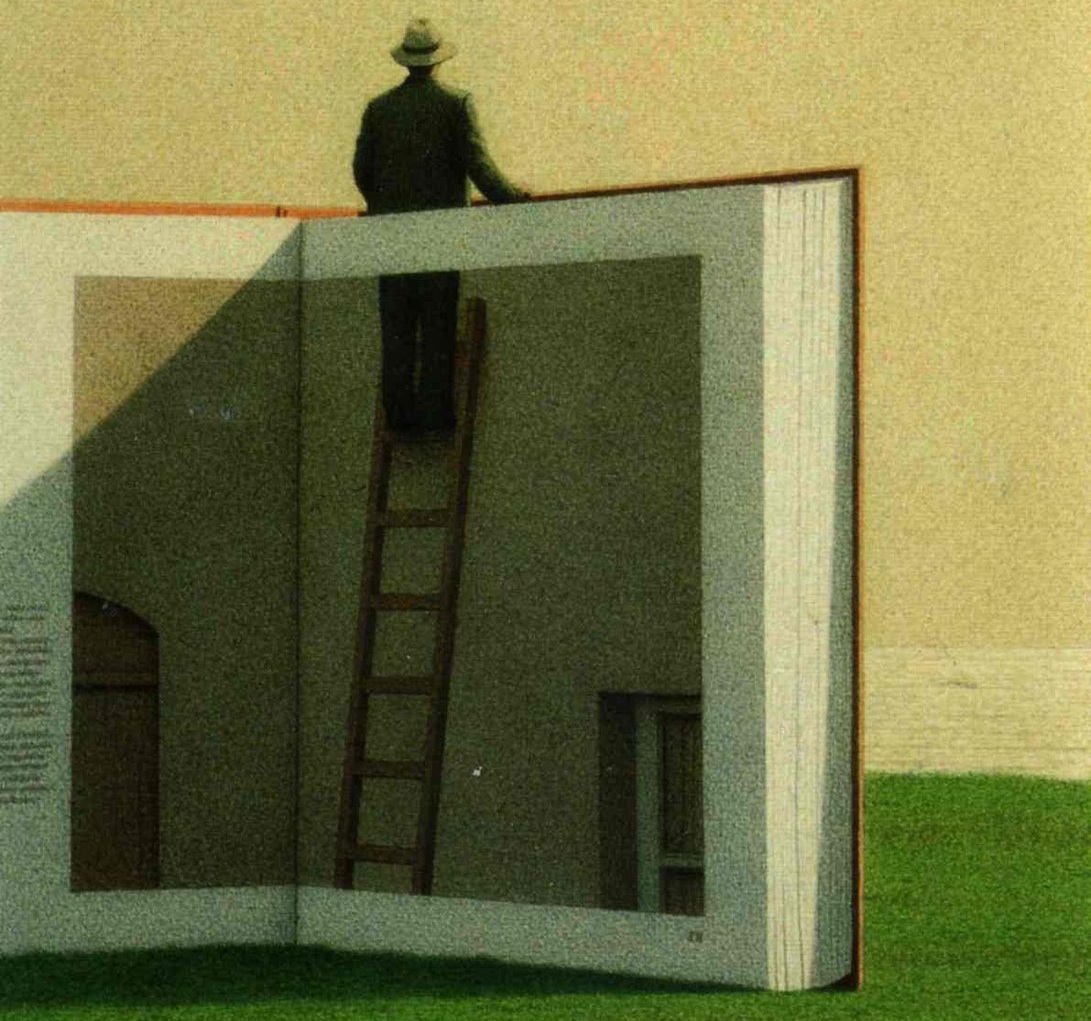
\includegraphics[width=\paperwidth,height=\paperheight]{img/summary/part.jpg}}
\part{What's next?}
}

\begin{frame}{What's next?}
	\begin{itemize}
		\item Updating to more recent JUnit version is easy
		\item Old tests will still run
		\item New tests will benefit from new features
		\item Old tests can be simplified little by little
		\item<alert@2> Try it out!
	\end{itemize}
\end{frame}

\begin{frame}{Try it out!}

	\url{http://www.junit.org/}\hspace{2.1cm}\url{http://hamcrest.org/}\par
	\url{https://github.com/marcphilipp/junit-4x-presentation}\par
	\vskip+1em

	\begin{beamercolorbox}[sep=1em]{blockbackground} 
		In theory, there is no difference between theory and practice.\\
		But, in practice, there is.\par\vskip-.5em
		\hfill\scriptsize Jan L. A. van de Snepscheut/Yogi Berra
	\end{beamercolorbox}\vskip+.5em

        \begin{block}{Nicole Rauch}
	\begin{description}[Twitter]
		\item[Mail]    \href{mailto:nicole.rauch@msg-gillardon.de}{\texttt{nicole.rauch@msg-gillardon.de}}
		\item[Twitter] \href{http://twitter.com/nicolerauch}{\texttt{@nicolerauch}}
	\end{description}
        \end{block}

        \begin{block}{Marc Philipp}
	\begin{description}[Twitter]
		\item[Mail]    \href{mailto:marc@andrena.de}{\texttt{marc@andrena.de}}
		\item[Twitter] \href{http://twitter.com/marcphilipp}{\texttt{@marcphilipp}}
	\end{description}
        \end{block}
\end{frame}

\begin{frame}{Many Matchers -- Many Classes}
	\begin{block}{Problem}
		\begin{itemize}
			\item Lots of matcher classes with static methods we would like to import
			\item Requires manual setup of preferences in IDE
			\item \dots for all developers!
		\end{itemize}
	\end{block}
	\begin{block}{Solution}
		Generate your own matcher library
	\end{block}
\end{frame}

\begin{frame}[fragile]{Generating a Custom Matcher Library}
	\begin{enumerate}
		\item Configuration in XML
			\lstinputlisting[language=XML,firstline=2]{java/EffectiveJUnit/src/de/andrena/junit/hamcrest/matchers.xml}
		\item Run \texttt{org.hamcrest.generator.config.XmlConfigurator}
		\item Combines all \texttt{@Factory} methods into a single generated class:
			\javainputlisting[firstline=7]{hamcrest}{Matchers}
	\end{enumerate}
\end{frame}

